\chapter{Implementation} \label{cha:chapter3}

\todo{split chapter section into design \& implementation}

\section{Technology Choices} \label{sec:chap3:technology}
This section will discuss choices that have been made throughout the project regarding technology used and justifications for their usage.

\subsection{Rust} \label{sec:chap3:technology:rust}
There were a few requirements when choosing an appropriate programming language for this project:
\begin{enumerate} 
    \item Performance: There are two aspects to performance within this project. Performance considerations and optimization are vital on IOT devices themselves, due to their limited on-board processing power. On the other hand, while performance on servers is definitely important, it is significantly easier to scale server-performance, by simply adding more servers (horizontal scaling) or by improving the hardware of any individual server (vertical scaling), than it is to improve performance of an IoT device. This is especially true of an IoT device that is already deployed.
    \item Stability: Another important requirement when choosing a language is the stability of code written in the language. This does not necessarily mean that code written in any language is inherently unstable. This requirement is more of a consideration about if a language enables and encourages a programmer to write code that is memory-safe and handles errors correctly. This is important in an IoT environment, as devices are expected to run for long periods. What is the point of a security camera if it's software crashes every couple days, due to an obscure memory out of bounds error? 
    \item Security: While no language is inherently "hack-proof" or secure, there are ways a language can encourage behaviors that can lead to better outcomes in security. A blog-post by the "Microsoft Security Response Centre" states that 70\% of all vulnerabilities assigned a CVE (Common Vulnerabilities and Exposures) each year are due to memory corruption errors \cite{ProactiveApproachToSecureCode}. In the post the languages "C" and "C++" are specifically referred to as being part of this problem. As mentioned in subsection ~\ref{sec:chap2:security}, security is of particular importance in smart home systems, so ensuring a method or language that enables secure code is chosen is of particular importance. 
    \item Ease of Use and Comfort: While not particularly important in the final product, having a language that is easy to develop in can make the developer experience easier and can lead to faster iteration on ideas, perhaps leading to a better final result. That being said, developer familiarity with a language can more than make up this difference. A seasoned C++ developer will be able to iterate faster and produce a better product in C++, than if they are using an "easy" language, that they are not as familiar with.
\end{enumerate}\todo{not sure I like the list style here}
After some deliberation, the language that was chosen for this project was Rust. While C/C++'s performance rivals and often surpasses Rust, the difference is often quite marginal \cite{PerformanceEvalOnMicrocontroller}, due to all three being compiled to machine code. What makes Rust different, is its headline feature, known as the "borrow checker". While the details of the borrow checker are out of scope of this paper, it can ensure that at compile-time, the code is memory safe. While there are ways to circumvent this (using the "unsafe" keyword), this has to be explicitly done. Due to the code being guaranteed memory safe at compile time, outside the aforementioned unsafe blocks, Rust code is known for its ability to run long-term without running into crashes. Additionally, Rust code is a popular choice for embedded devices, due to being able to compile without a standard library (this has to be enabled), giving it flexibility in a project such as this.

I have decided to use Rust for both the Server and Clients. While Rust might be a somewhat obvious choice for IoT clients, it is less so for servers. Due to the "borrow checker", while Rust might be safe, it is often said to be harder to write than traditional languages. This makes it more questionable as the primary language for the server, due to it being a less constrained platform (view performance section above). While servers are theoretically almost infinitely horizontally scalable, in practice this is often not the case, especially in a smart-home's case, as they have to fit in someone's home and generally should be affordable. Therefore, ensuring that the server can run on as many devices as possible, be it a Raspberry-Pi, or a modern desktop, is an important goal to strive for. The "difficulty" aspect of Rust can be largely counteracted by personal familiarity with the language. Additionally, having a stable server is very important, especially since all IoT devices will need to frequently communicate with this server, an aspect which Rust excels at. Rust also has a thriving community of libraries (known as crates), which using the language gives access to. For these reasons I have chosen Rust as the primary programming language of the Server and Client parts of this project.

\subsection{gRPC} \label{sec:chap3:technology:grpc}
gRPC is an RPC implementation released by Google in 2015. It uses Protocol Buffers (protobufs) as an interface definition language (IDL), to define services on servers, that clients can then call, such as any RPC library. The server runs a gRPC server and the client runs the gRPC client \cite{grpcHomepage}. Protobufs are compiled to many different languages, with many different libraries available for these languages, that automate much of the process. In a performance comparison between REST, gRPC, websockets, GraphQL, gRPC came out ahead in many different metrics \cite{reviewOfInternetProtocols}. These include: 
\begin{itemize}
    \item inserting one value into a database
    \item fetching one value from a database 
    \item fetching one hundred elements  
\end{itemize}
in both native and containerized tests. In fact, gRPC was the most performant internet communication protocol in all metrics apart from memory usage.

Due to its performance and cross-language support I have chosen gRPC as the internet communication protocol for this project. The specific library used for this project is known as "Tonic". Tonic is a Rust gRPC crate that includes both a gRPC server and client. It also utilizes "prost" to compile protobuf files into Rust code, without having to interface the protobuf compiler itself. All protobuf files are compiled as a compilation step of the server and client, eliminating the need for external build scripts (this is only partially true, view Sub Section~\ref{sec:chap3:server:protoBufs}).

\subsection{Typescript \& VueJS} \label{sec:chap3:technology:ts}
While a Command Line Interface (CLI) frontend, written in Rust, will be made available, the main focus will be on the Graphical User Interface (GUI). To ensure that it can run on a variety of systems and is relatively easy to create, it will be web based, using Javascript at runtime. However, it will be written in Typescript. Typescript is a superset of Javascript, that compiles to Javascript and leaves no trace of types behind. Typescript provides a robust type-system, including, but not limited to \cite{understandingTypescript}:
\begin{itemize}
    \item Structural type equivalence, instead of Javascript's by-name type equivalence
    \item Types and concepts for object-based programming
    \item Type operators
\end{itemize}
All of these, while not guaranteeing that the program will be type-safe at runtime, help a developer design more robust and long term solutions generally associated with statically typed languages.

In conjunction with Typescript a web-development framework will be used. Web frameworks are libraries for Javascript that allow easier development of websites and web apps, often incorporating HTML (HyperText Markup Language) and CSS (Cascading Style Sheets) code into Javascript code. They also provide reactivity, meaning that if a variable changes in the code, that change can easily be reflected on the site. This can be done in most frameworks by simply using the variable in the HTML code, something that standard HTML does not support (methods of doing this differs between frameworks).

Most of the choice between different web-frameworks comes down to personal preference and familiarity with a framework. That being said there can be performance differences between different frameworks, that could make a difference on some systems. While there is a lack of formal experiments on framework performance, an informal experiment \cite{performanceComparisonJS} showed that while there is a performance difference between different frameworks, it should not be the primary decision maker. When the difference when creating 1000 rows between vanilla JavaScript and VueJS is 32 milliseconds, the disparity will not be noticeable to the end user. For this reason, and personal familiarity with the framework, I have decided to use VueJS as the frontend development framework for this project.

\subsection{Raspberry Pi} \label{sec:chap3:technology:raspi}
\todo{write this}

\section{Server \& Hub} \label{sec:chap3:server}
Due to the server being the largest part of this project, and practically being a requirement for testing the client and frontend functionality, this will be focused on first. This section will describe defining and compiling protobuf files for API endpoints, server startup, how IOT devices are registered, security mechanisms and how concurrency was handled within the server. 

\subsection{Protocol Buffers and Tonic} \label{sec:chap3:server:protoBufs}
\todo{I think this section is probably fine, just talk some more about what these protobufs and method stubs will be used for}
Protobufs are defined within ".proto" files. They use a fairly basic syntax, where the user can define a service using the "service" keyword. A service can contain many functions which a client can call, these are defined using the "rpc" keyword. You can also define the arguments this function takes and what it returns. Structs are defined using the "message" keyword, where each field is separated by a semicolon. Fields can have multiple modifiers, including optional, repeated and map. Repeated marks a field as possibly being a list, or array structure. Map marks a field as being a map data structure. Finally, messages from other files can be imported, using the import keyword and then giving the file-name. \cite{protobufDocs} For an example of a protobuf file view \textbf{\textit{protos/iot/registrationService.proto}}:

\begin{lstlisting}[language=protobuf3, style=boxed]{iot/registrationService.proto}
syntax = "proto3";
package iot.registration;
import "types.proto";

service RegistrationService {
    rpc Register(
        RegistrationRequest
    ) returns (RegistrationResponse);
};

message RegistrationRequest {
    string public_key = 1;
    string name = 2;
    repeated iot.types.DeviceCapabilityStatus capabilities = 3;
}

message RegistrationResponse {
    string public_key = 1;
    string client_id = 2;
    string certificate = 3;
}
\end{lstlisting}

Here we define a service called "RegistrationService", with a function called Register. This function is called by IOT clients when they first attempt to connect to the server which takes a RegistrationRequest as a parameter and returns a RegistrationResponse. The file also defines two "messages", the aforementioned RegistrationRequest and RegistrationResponse. While most of the fields within them are fairly obvious, RegistrationRequest.capabilities warrants further explanation.
    This field is repeated, meaning it is an array data structure. This array contains the type DeviceCapabilityStatus, which is defined in iot.types. We can see this type is imported at the top of the file, from "types.proto". This is the definition of DeviceCapabilityStatus:

\begin{lstlisting}[language=protobuf3, style=boxed]{iot/types.proto}
message DeviceCapabilityStatus {
    bool available = 1;
    string capability = 2;
}
\end{lstlisting}

In summary, if an IOT device wants to register with this server, they will need to call the Register server stub. The server stub takes one parameter, the RegistrationRequest message. This message requires the client to give it's public key, it's display name and an array of "DeviceCapabilityStatus". The Register function then returns a RegistrationResponse. 

To compile these server stubs to Rust we will be using the aforementioned Rust "Tonic" crate. To do this first we must add the "Tonic" crate to our project, then add "tonic-build" to our build dependencies (view Cargo Documentation). We then create a build.rs file, which is run when the Rust compiler (Cargo) builds the program. You can view the file \textbf{\textit{backend/build.rs}} below:

\begin{lstlisting}[language=Rust, style=boxed, showstringspaces=false]{backend/build.rs}
fn main() -> Result<(), Box<dyn std::error::Error>> {
    tonic_build::compile_protos(
        "../proto/iot/types.proto"
    )?;
    tonic_build::compile_protos(
        "../proto/iot/registrationService.proto"
    )?;
    tonic_build::compile_protos(
        "../proto/iot/requestUpdateService.proto"
    )?;
    tonic_build::compile_protos(
        "../proto/iot/deviceControlService.proto"
    )?;

    tonic_build::configure()
        .type_attribute(
            ".", 
            "#[derive(serde::Deserialize, serde::Serialize)]"
        )
        .compile(
            &[
                "../proto/frontend/registrationService.proto",
                "../proto/frontend/frontendTypes.proto",
                "../proto/iot/types.proto",
                "../proto/frontend/deviceControlService.proto",
            ],
            &["../proto/frontend", "../proto/iot"],
        )?;
    Ok(())
}
\end{lstlisting}

In line 2-13 we are telling tonic\_build, using prost under the hood (which in turn calls the protobuf compiler), to compile the files required for Device \& Server communication. We do this by calling the \textit{compile\_protos} function. The files in the folder \textit{proto/iot} are the ones used by IOT devices. This is quite simple to use, however is technically a build script, making the statement in subsection~\ref{sec:chap3:technology:grpc} partially untrue. Line 15-28 are where frontend protobuf files are compiled. These require the traits (Rust equivalent to interfaces in other languages) "Serialize" and "Deserialize" to be implemented for all structs compiled from the files. We therefore require this special syntax when compiling them. For more information on why they need these traits, view subsection~\ref{sec:chap3:frontend:json}.

Finally, protobuf server-stubs and messages can be imported into Rust using a macro provided by tonic. View below how \textbf{\textit{backend/src/server/registration.rs}} imports the \textit{protos/iot/registration.proto} file:

\begin{lstlisting}[language=Rust, style=boxed]{server/registration.rs}
use crate::types::types;
pub mod registration_service {
    tonic::include_proto!("iot.registration");
}
\end{lstlisting}

In order to import the compiled protbuf file, we simply call the "include\_proto" macro (it being a macro is indicated by the \textbf{!}). Note that we need to import the types module first, as this module contains the compiled \textit{protos/iot/types.proto} file, which is imported by \textit{registration.proto}. Additionally, instead of giving the file path to the protobuf file, we simply give the module name, which is also defined in the protobuf file.

\subsection{Server Start Up} \label{sec:chap3:server:startup}
This section will describe what is done when the server first starts. It will give a general overview of startup and the details of starting a gRPC and HTTP server in Rust. For more details, view the main function within \textit{\textbf{/backend/src/server/server.rs}}.

Startup of the server is currently quite simple:

\begin{figure}[h]
\caption{Simplified Diagram of Server Startup}
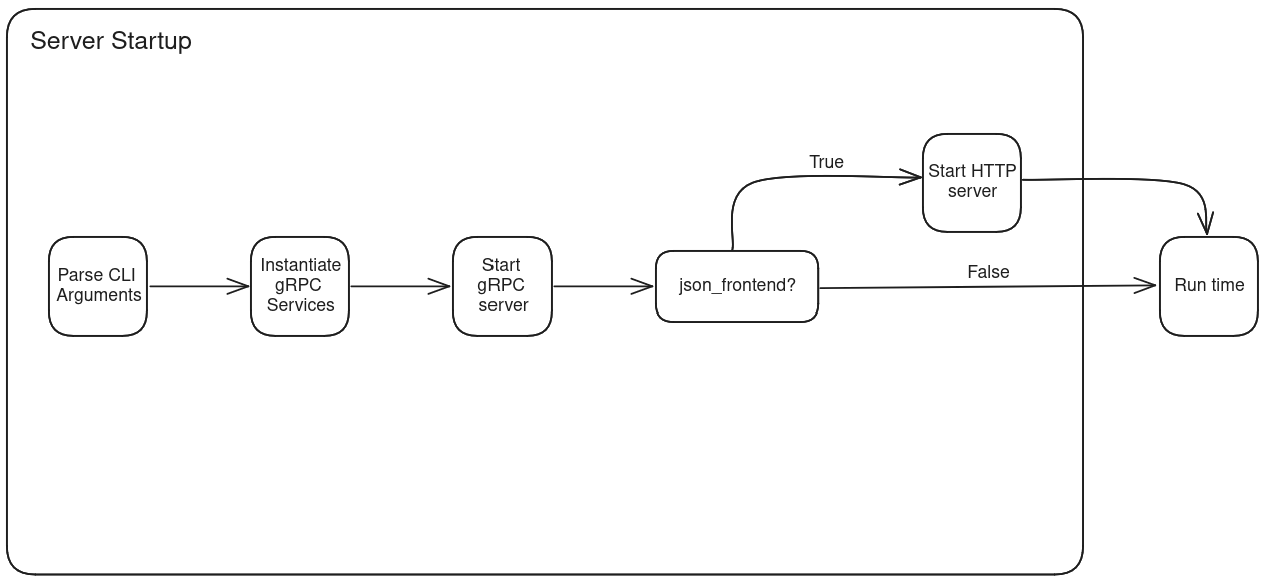
\includegraphics[width=\textwidth]{server_startup}
\end{figure}

\subsubsection{Command Line Arguments}
Command line (CLI) arguments are parsed using a Rust library called "Clap". Currently the only commandline argument that can be passed is running the optional HTTP server, which enables using JSON for the frontend (view subsection~\ref{sec:chap3:frontend:json}), however there are plans to include other arguments, such as giving an IP address or Port for the gRPC server to run on as an argument. Currently, the computer's IP address is discovered automatically using a crate called "local-ip-address". 

\subsubsection{Creating gRPC Services}
Next gRPC services are instantiated. GRPC services in Rust take the form of structs that implement the trait (interface) defined as a service within a protbuf file. Take for example, the "RegistrationService" from \textbf{\textit{protos/iot/registrationService.proto}}, defined in subsection~\ref{sec:chap3:server:protoBufs}:
\begin{lstlisting}[language=protobuf3, style=boxed, showstringspaces=false]{}
service RegistrationService {
    rpc Register(
        RegistrationRequest
    ) returns (RegistrationResponse);
};
\end{lstlisting}

This is implemented on a struct in Rust like this (code snippet from \textit{\textbf{backend/src/server/registration.rs}}):
\begin{lstlisting}[language=Rust, style=boxed, showstringspaces=false]{}
use self::registration_service
    ::registration_service_server::RegistrationService;

#[async_trait]
impl RegistrationService for ClientRegistrationHandler {
    async fn register(
        &self,
        request: tonic::Request<
            self::registration_service::RegistrationRequest
        >,
    ) -> RPCFunctionResult<
        self::registration_service::RegistrationResponse
    > {
        //code goes here
    }
}
\end{lstlisting}

Where "RegistrationService" is the trait we are implementing and "ClientRegistrationHandler" is the name of the struct it is being implemented on. If the trait is implemented correctly, this struct is now a service and, after being handed to the gRPC server struct, this function can then be called using an RPC through gRPC. In other words, any gRPC client that is connected to this gRPC server can now call this function, as long as their programming language supports it.

\subsubsection{Starting the gRPC Server}
After implementing all services defined in the protobuf files on appropriate structs, the gRPC server can now be started. This is done in the following code snippet from \textit{\textbf{/backend/src/server/server.rs}}:
\begin{lstlisting}[language=Rust, style=boxed, showstringspaces=false]{}
use registration_service_server::RegistrationServiceServer;

let registration_service =
    registration::ClientRegistrationHandler::new();
let grpc_server = tonic::transport::Server::builder()
    .add_service(
        RegistrationServiceServer::new(
            registration_service,
        )
    )
    .serve_with_shutdown(
        grpc_address,
        tokio::signal::ctrl_c().map(drop)
    )
    .await;

println!("Started GRPC Server on {}", grpc_address);
\end{lstlisting}
\textit{Note that the above code snippet is abbreviated for readability, it is however still valid Rust code and gives a good representation of what is done in server.rs.} 

The Server struct we are instantiating on line 1 comes from the transport module within the tonic crate. We invoke the builder method on the Server struct, a very common pattern within the Rust ecosystem. In fact, the same pattern is used instantiate a new IoT device in the client library for this project (view section~\ref{sec:chap3:devicelib}). After invoking the builder method, which returns a new Server struct, we add structs that implement the aforementioned services to it, using the "add\_service" method. In our case, we want to hand it a "RegistrationServiceServer" struct, provided by the protobuf file. The "new" method on the "RegistrationServiceServer" takes one argument, which is a struct that implements the "RegistrationService" trait, which is the trait we implemented on our ClientRegistrationHandler earlier. We therefore hand it an instance of the "ClientRegistrationHandler", held in the variable "registration\_service".

The "server\_with\_shutdown" method consumes the Server struct and runs the server, on the address handed to it in the parameter. In this case it is the variable "grpc\_address", which is a string which contains the device's IP address and a port. The second parameter simply tells Rust to drop the gRPC server (shutdown and gracefully free the memory associated with it) when the key combination crtl-c is pressed. This is an easy way to implement this behavior in Rust when working with multiple threads (view subsection~\ref{sec:chap3:server:threads}).

Once we have added all services to the Server struct, it must be awaited using the "await" keyword. For more information on how this works view subsection~\ref{sec:chap3:server:threads}.  

\subsubsection{Starting the HTTP Server}
Starting the HTTP server works almost the same as the gRPC server, using the same builder pattern. However, this time instead of using the Tonic crate, we are using a crate named "Actix", a self-described "powerful, pragmatic, and extremely fast web framework for Rust" \cite{actixWebsite}. View part of the "run\_json\_frontend" function, found in the file \textbf{\textit{backend/src/server/server.rs}} below:
\begin{lstlisting}[language=Rust, style=boxed, showstringspaces=false]{}
const JSON_ADDRESS: &str = "localhost:50052";

let result = actix_web::HttpServer::new(move || {
    actix_web::app::App::new()
        .app_data(web::Data::new(json_state.clone()))
        .service(json_registration::json_registration)
})
.bind(JSON_ADDRESS)?
.run()
.await;

println!("Successfully Started JSON API Layer on {JSON_ADDRESS}");
\end{lstlisting}
\textit{Note that the above code snippet is abbreviated for readability, it is however still valid Rust code and gives a good representation of what is done in server.rs.} 

Due to this builder function requiring more Rust specific knowledge to understand, it will be simplified here. It is functionally the same as the one seen from Tonic. First we create a new HTTPServer struct from the actix\_web module. We then hand it our services using the "service" method. What is different here, is that we are actually handing it callback functions, instead of structs with traits implemented. To view an example of these services, view subsection~\ref{sec:chap3:server:registration}. From there we bind this server to the constant string JSON\_ADDRESS. This is an IP Address defined at compile time, the definition however is found above the web server. The server is running on localhost, as it is meant for communication with the web frontend. We then call the run method and await the result. In reality the server is being awaited on a different thread than the gRPC server, so the two can run concurrently, this is not shown in the above code snippet. 

For code beyond the above provided abbreviated snippets view the file \textbf{\textit{backend/src/server/server.rs}}, which contains the main function for the server.

\subsection{Device Registration} \label{sec:chap3:server:registration} 

\subsection{Security} \label{sec:chap3:server:security}

\subsection{Threads \& Concurrency} \label{sec:chap3:server:threads}


\section{Device Library} \label{sec:chap3:devicelib}
\section{Example Device} \label{sec:chap3:deviceexample}
\section{Networking}

\section{Web \& CLI Frontend} \label{sec:chap3:frontend}
\subsection{Using JSON for the Frontend API} \label{sec:chap3:frontend:json}
Write about here:
- Show Json service in Rust
- Why its bound on localhost
- Why protobuf compiler needs Serialize and Deserialize on these structs
